\subsubsection{XAI Wav2Vec2}

Ahora que tenemos el resultado del modelo (el Wav2Vec2 fine-tuneado), vamos a explicar que características y que parte del espectrograma de Mel del audio son las más influyentes y en que sentido.

Sin embargo ahora nos encontramos con el problema principal de este modelo que es que como entrada recibe un embedding, entonces, no podemos aplicar técnicas de XAI directamente al modelo. Otro problema que tenemos es que el código que tenemos de extracción de características saca muchísimas características y de ciertas características no solo saca un valor escalar sino que también saca un vector con sus valores en cada instante.

Para solucionar estos problemas hemos hecho dos cosas. La primera es que agruparemos las características en cinco grupos en función de sus características y lo que representan. Con esto nos quedan las siguientes agrupaciones:

\begin{enumerate}
 \item Energía: rms, silence ratio, zcr, skewness, kurtosis. Este grupo son las características que se centran en la energía del audio.
 \item Espectrales: spectral centroid, spectral bandwidth, spectral rolloff, spectral flatness, hnr. Este grupo son las características que miden la distribución de la energía en el ámbito de la frecuencia.
 \item Pitch: pitch mean, pitch std. Este grupo son las características %falta completar
 \item Formantes:  f1 mean, f2 mean, f3 mean. Este grupo son las características que describen la estructura vocal.
 \item MFCC: mfcc1 mean, mfcc2 mean,  mfcc3 mean, mfcc4 mean,  mfcc5 mean, mfcc6 mean,  mfcc7 mean, mfcc8 mean,  mfcc9 mean, mfcc10 mean,  mfcc11 mean, mfcc12 mean,  mfcc13 mean. Este grupo de características capturan %falta completar
	\end{enumerate}

La segunda cosa que se ha hecho ha sido desarrollar modelos sencillos que imiten el comportamiento del modelo. Para esto hemos hecho 6 modelos distintos. Cinco de ellos son regresiones logísticas, uno para cada grupo de características y una CNN muy simple para los espectrogramas.

Una vez tenemos los surrogate models hechos, ahora les vamos a aplicar técnicas de ia explicable. La primera técnica que aplicaremos a cada modelo de regresión es el Shap. Para cada modelo, esta técnica nos sacará dos gráficas, la primera es el impacto general de cada característica en la respuesta del modelo	y la segunda es el impacto de cada característica para un audio concreto. Con esto, vamos a ir explicando modelo por modelo.

\begin{enumerate}
 \item Energía: En este modelo podemos ver como la kurtosis y el silence ratio son las características que más influyen mientras que el rms tiene una influencia nula en la predicción.
 
 \begin{figure}[H]
	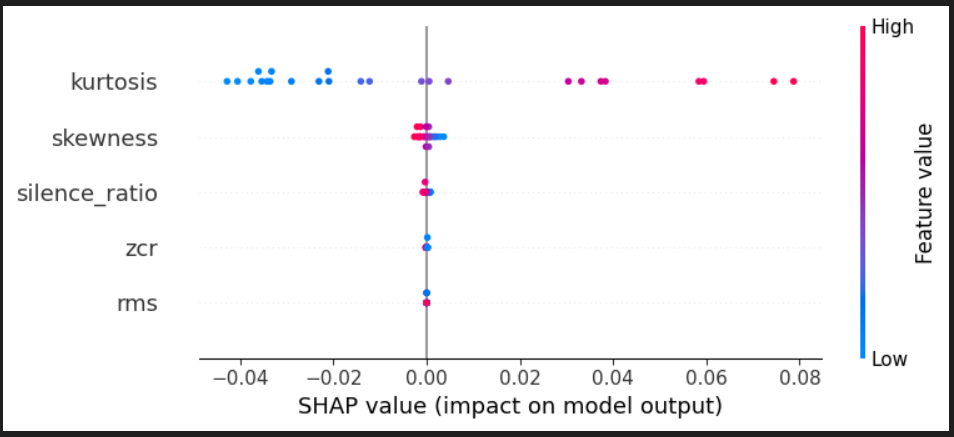
\includegraphics[width=\textwidth]{imagenes/Influencia_caracteristicas_energia_wav2vec2.png}
	\caption{Influencia general de las características.}
	\label{fig:Wav2Vec2}
 \end{figure}

 \begin{figure}[H]
	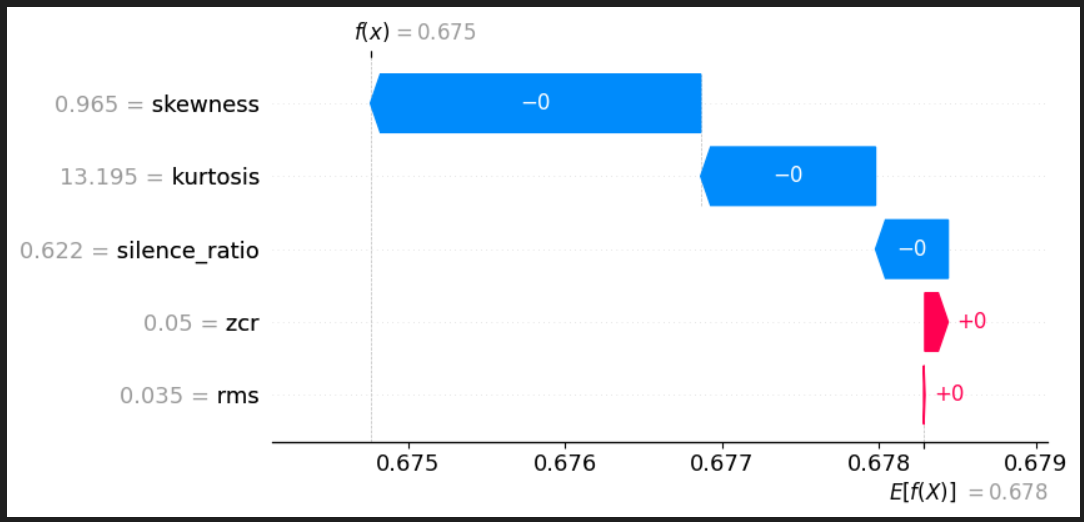
\includegraphics[width=\textwidth]{imagenes/Influencia_caracteristicas_energia_instancia_wav2vec2.png}
	\caption{Ejemplo concreto.}
	\label{fig:Wav2Vec2}
 \end{figure}

 \item Espectrales: En este modelo podemos ver como el spectral centroid es la característica dominante aunque seguida de cerca por el spectral rolloff y el spectral bandwidth. También se puede apreciar que el spectral flatness no tiene influencia en la predicción.
 
 \begin{figure}[H]
	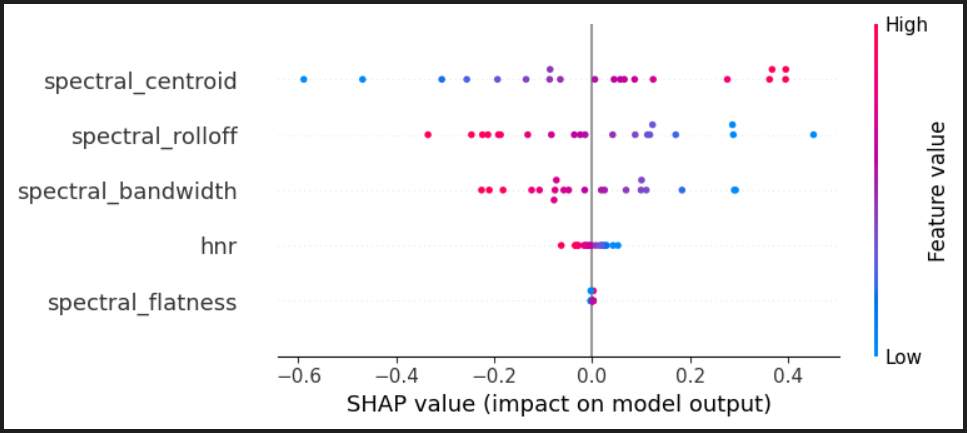
\includegraphics[width=\textwidth]{imagenes/Influencia_caracteristicas_espectrales_wav2vec2.png}
	\caption{Influencia general de las características.}
	\label{fig:Wav2Vec2}
 \end{figure}

 \begin{figure}[H]
	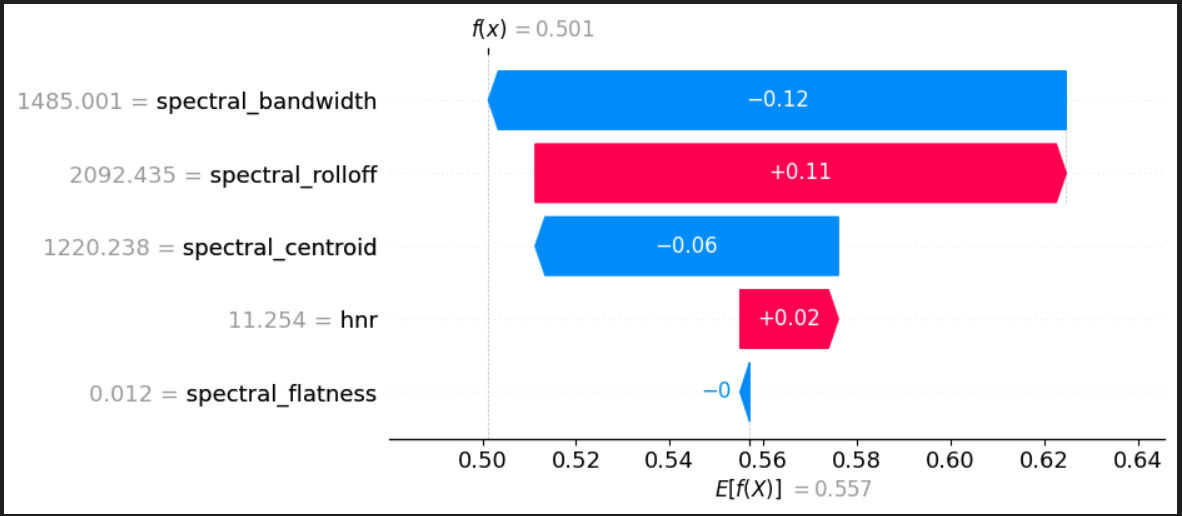
\includegraphics[width=\textwidth]{imagenes/Influencia_caracteristicas_espectrales_instancia_wav2vec2.png}
	\caption{Ejemplo concreto.}
	\label{fig:Wav2Vec2}
 \end{figure}
 
 \item Pitch: En este modelo hay un claro dominio por parte del pitch std en comparación con el pitch mean.
 
 \begin{figure}[H]
	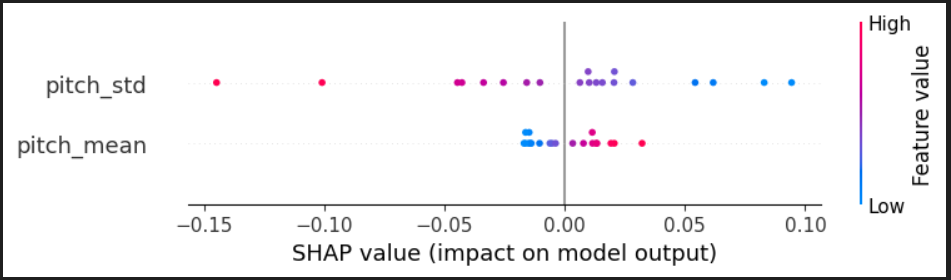
\includegraphics[width=\textwidth]{imagenes/Influencia_caracteristicas_pitch_wav2vec2.png}
	\caption{Influencia general de las características.}
	\label{fig:Wav2Vec2}
 \end{figure}

 \begin{figure}[H]
	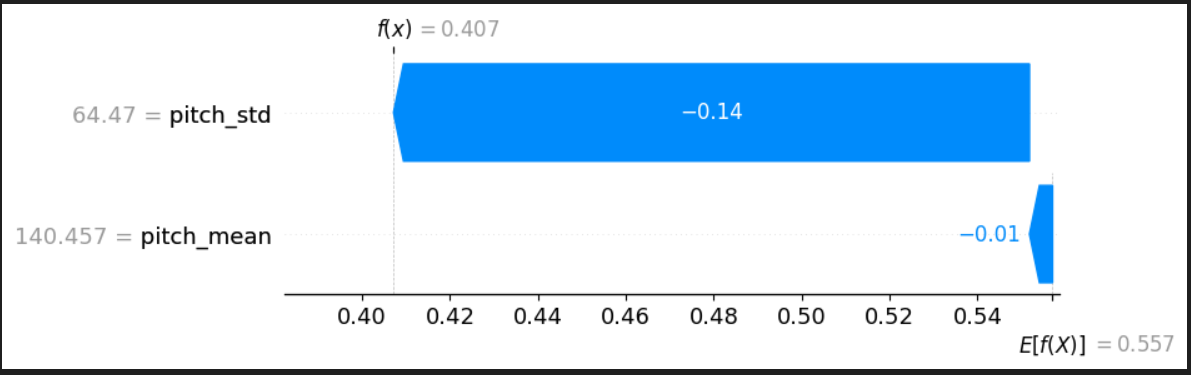
\includegraphics[width=\textwidth]{imagenes/Influencia_caracteristicas_pitch_instancia_wav2vec2.png}
	\caption{Ejemplo concreto.}
	\label{fig:Wav2Vec2}
 \end{figure}
 
 \item Formantes: En este modelo la f1 y la f3 tienen una influencia similar y muy superior a la de f2.
 
 \begin{figure}[H]
	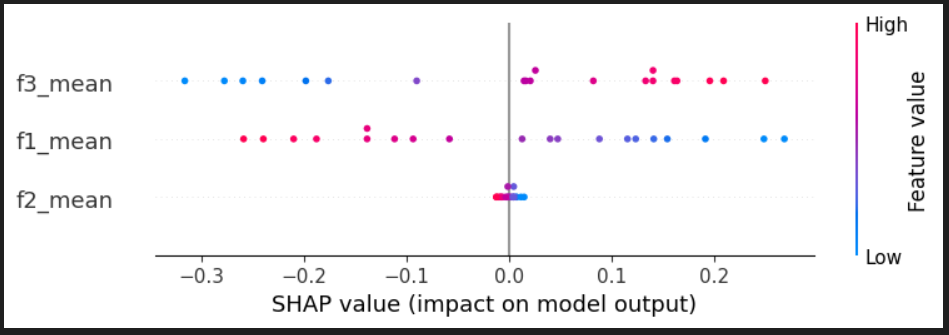
\includegraphics[width=\textwidth]{imagenes/Influencia_caracteristicas_formants_wav2vec2.png}
	\caption{Influencia general de las características.}
	\label{fig:Wav2Vec2}
 \end{figure}

 \begin{figure}[H]
	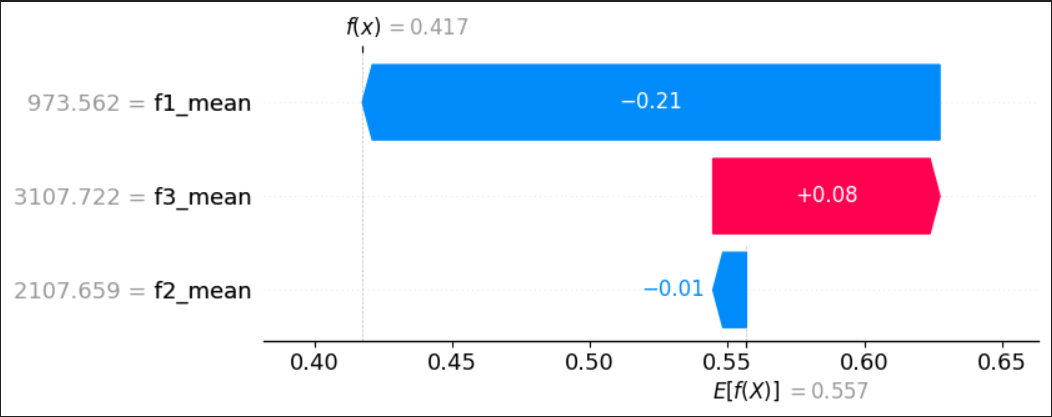
\includegraphics[width=\textwidth]{imagenes/Influencia_caracteristicas_formants_instancia_wav2vec2.png}
	\caption{Ejemplo concreto.}
	\label{fig:Wav2Vec2}
 \end{figure} 
 
 \item MFCC: %Completar texto y fotos
 
	\end{enumerate}

Ahora para las características, buscando también algo que complemente la explicación del Shap, vamos a usar Lime para explicar los mismos modelos y la misma instancia particular 

\begin{enumerate}
 \item Energía: En este modelo podemos ver como la kurtosis es la única característica que tiene un impacto relevante en la predicción del modelo. 
 
 \begin{figure}[H]
	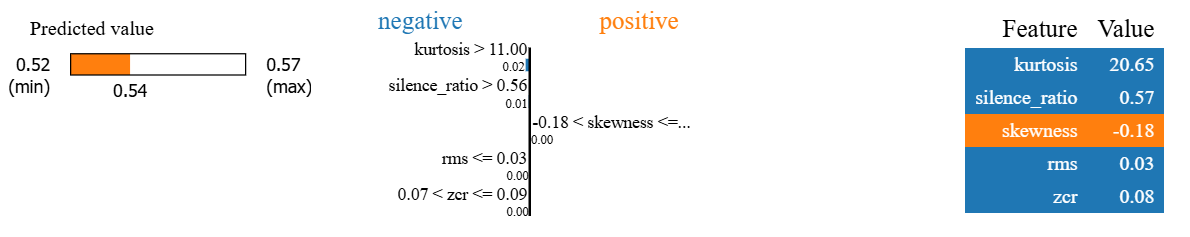
\includegraphics[width=\textwidth]{imagenes/Influencia_caracteristicas_energia_lime_wav2vec2.png}
	\caption{Influencia general de las características.}
	\label{fig:Wav2Vec2}
 \end{figure}

 \item Espectrales: En este modelo podemos ver como todas las características tienen algo de impacto, sin embargo predominan claramente el espectral bandwidth y el espectral centroid hacia reducir la predicción y el espectral rolloff hacia aumentarla
 
 \begin{figure}[H]
	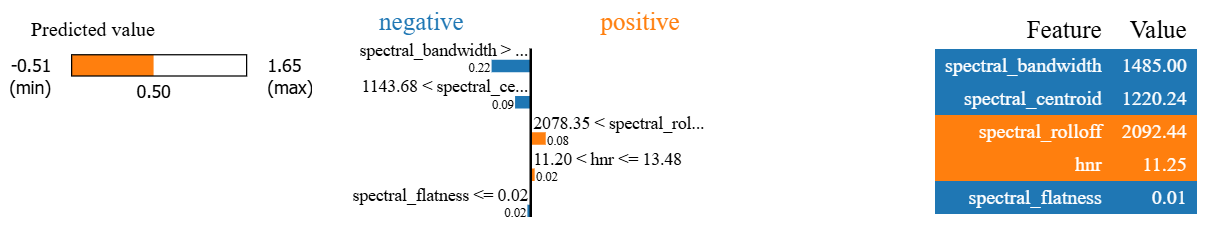
\includegraphics[width=\textwidth]{imagenes/Influencia_caracteristicas_espectrales_lime_wav2vec2.png}
	\caption{Influencia general de las características.}
	\label{fig:Wav2Vec2}
 \end{figure}
 
 \item Pitch: En este modelo se ve como el pitch std influye más que el pitch mean. Ambas características empujan la predicción hacia abajo.
 
 \begin{figure}[H]
	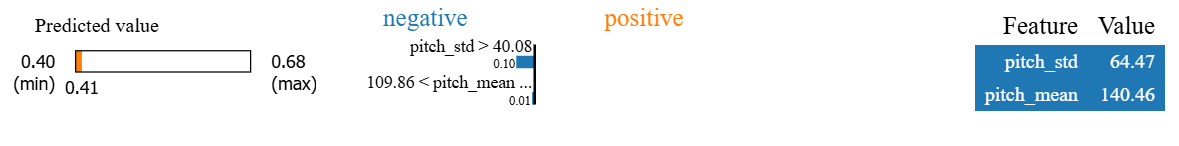
\includegraphics[width=\textwidth]{imagenes/Influencia_caracteristicas_pitch_lime_wav2vec2.png}
	\caption{Influencia general de las características.}
	\label{fig:Wav2Vec2}
 \end{figure}
 
 \item Formantes: En este modelo la f1 domina sobre las demás siendo la que más empuja la predicción hacia alguna dirección, en este caso, contribuye a reducirla mientras que la f3 la empuja hacia arriba aunque con menos fuerza de lo que la f1 lo hace hacia abajo.
 
 \begin{figure}[H]
	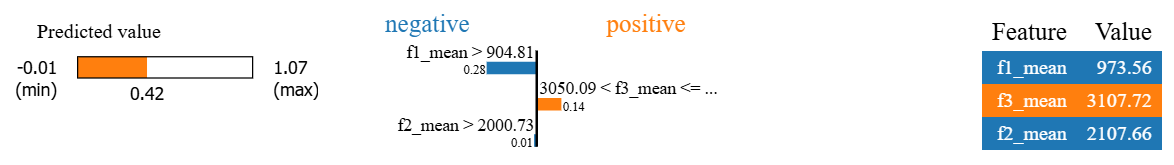
\includegraphics[width=\textwidth]{imagenes/Influencia_caracteristicas_formants_lime_wav2vec2.png}
	\caption{Influencia general de las características.}
	\label{fig:Wav2Vec2}
 \end{figure}
 
 \item MFCC: %Completar texto y fotos
 
	\end{enumerate}

Ahora que ya tenemos tanto el Shap como el Lime de todas las características de los audios, vamos a agregar los resultados de los cinco modelos para ver de forma general cuales son las características más influyentes a la hora de clasificar los audios en reales o generados.

Para esta tarea se ha hecho lo siguiente, primero calculamos la importancia promedio de cada característica usando sus valores Shap, luego calculamos la importancia de cada grupo de características y con esto podemos promediar la importancia de cada característica entre todos los grupos de características. Por último los ordenamos de mayor a menor importancia y los mostramos.

%Gráfica del Shap
%Analizar resultados gráfica

Para Lime hacemos exactamente lo mismo.

%Gráfica del Lime
%Analizar resultados gráfica

Ahora pasamos al sexto surrogate model, una CNN muy simple que se compone solo de una capa convolucional y una capa de pooling. Además se simplificará la entrada agrupando todas las bandas de frecuencia en 8 bandas solamente. Esto se hace para evitar que se produzca un sobreajuste ya que tenemos muy pocos audios.

Para los espectrogramas usaremos cuatro modelos de XAI siendo estos Shap, Lime, Integrated Gradients y Grad Cam. Para las cuatro técnicas la salida se mostrará superponiendo la salida del modelo de XAI con el espectrograma de Mel del audio.

SHAP

LIME

INTEGRATED GRADIENTS

GRAD CAM

Análisis de resultados y conclusiones

Cosas que faltan por hacer:
Sacar la explicación general de los modelos de XAI para los espectrogramas 
Combinación los espectrogramas con las características y sacar la correlación entre las explicaciones.
